\begin{figure}
\centering
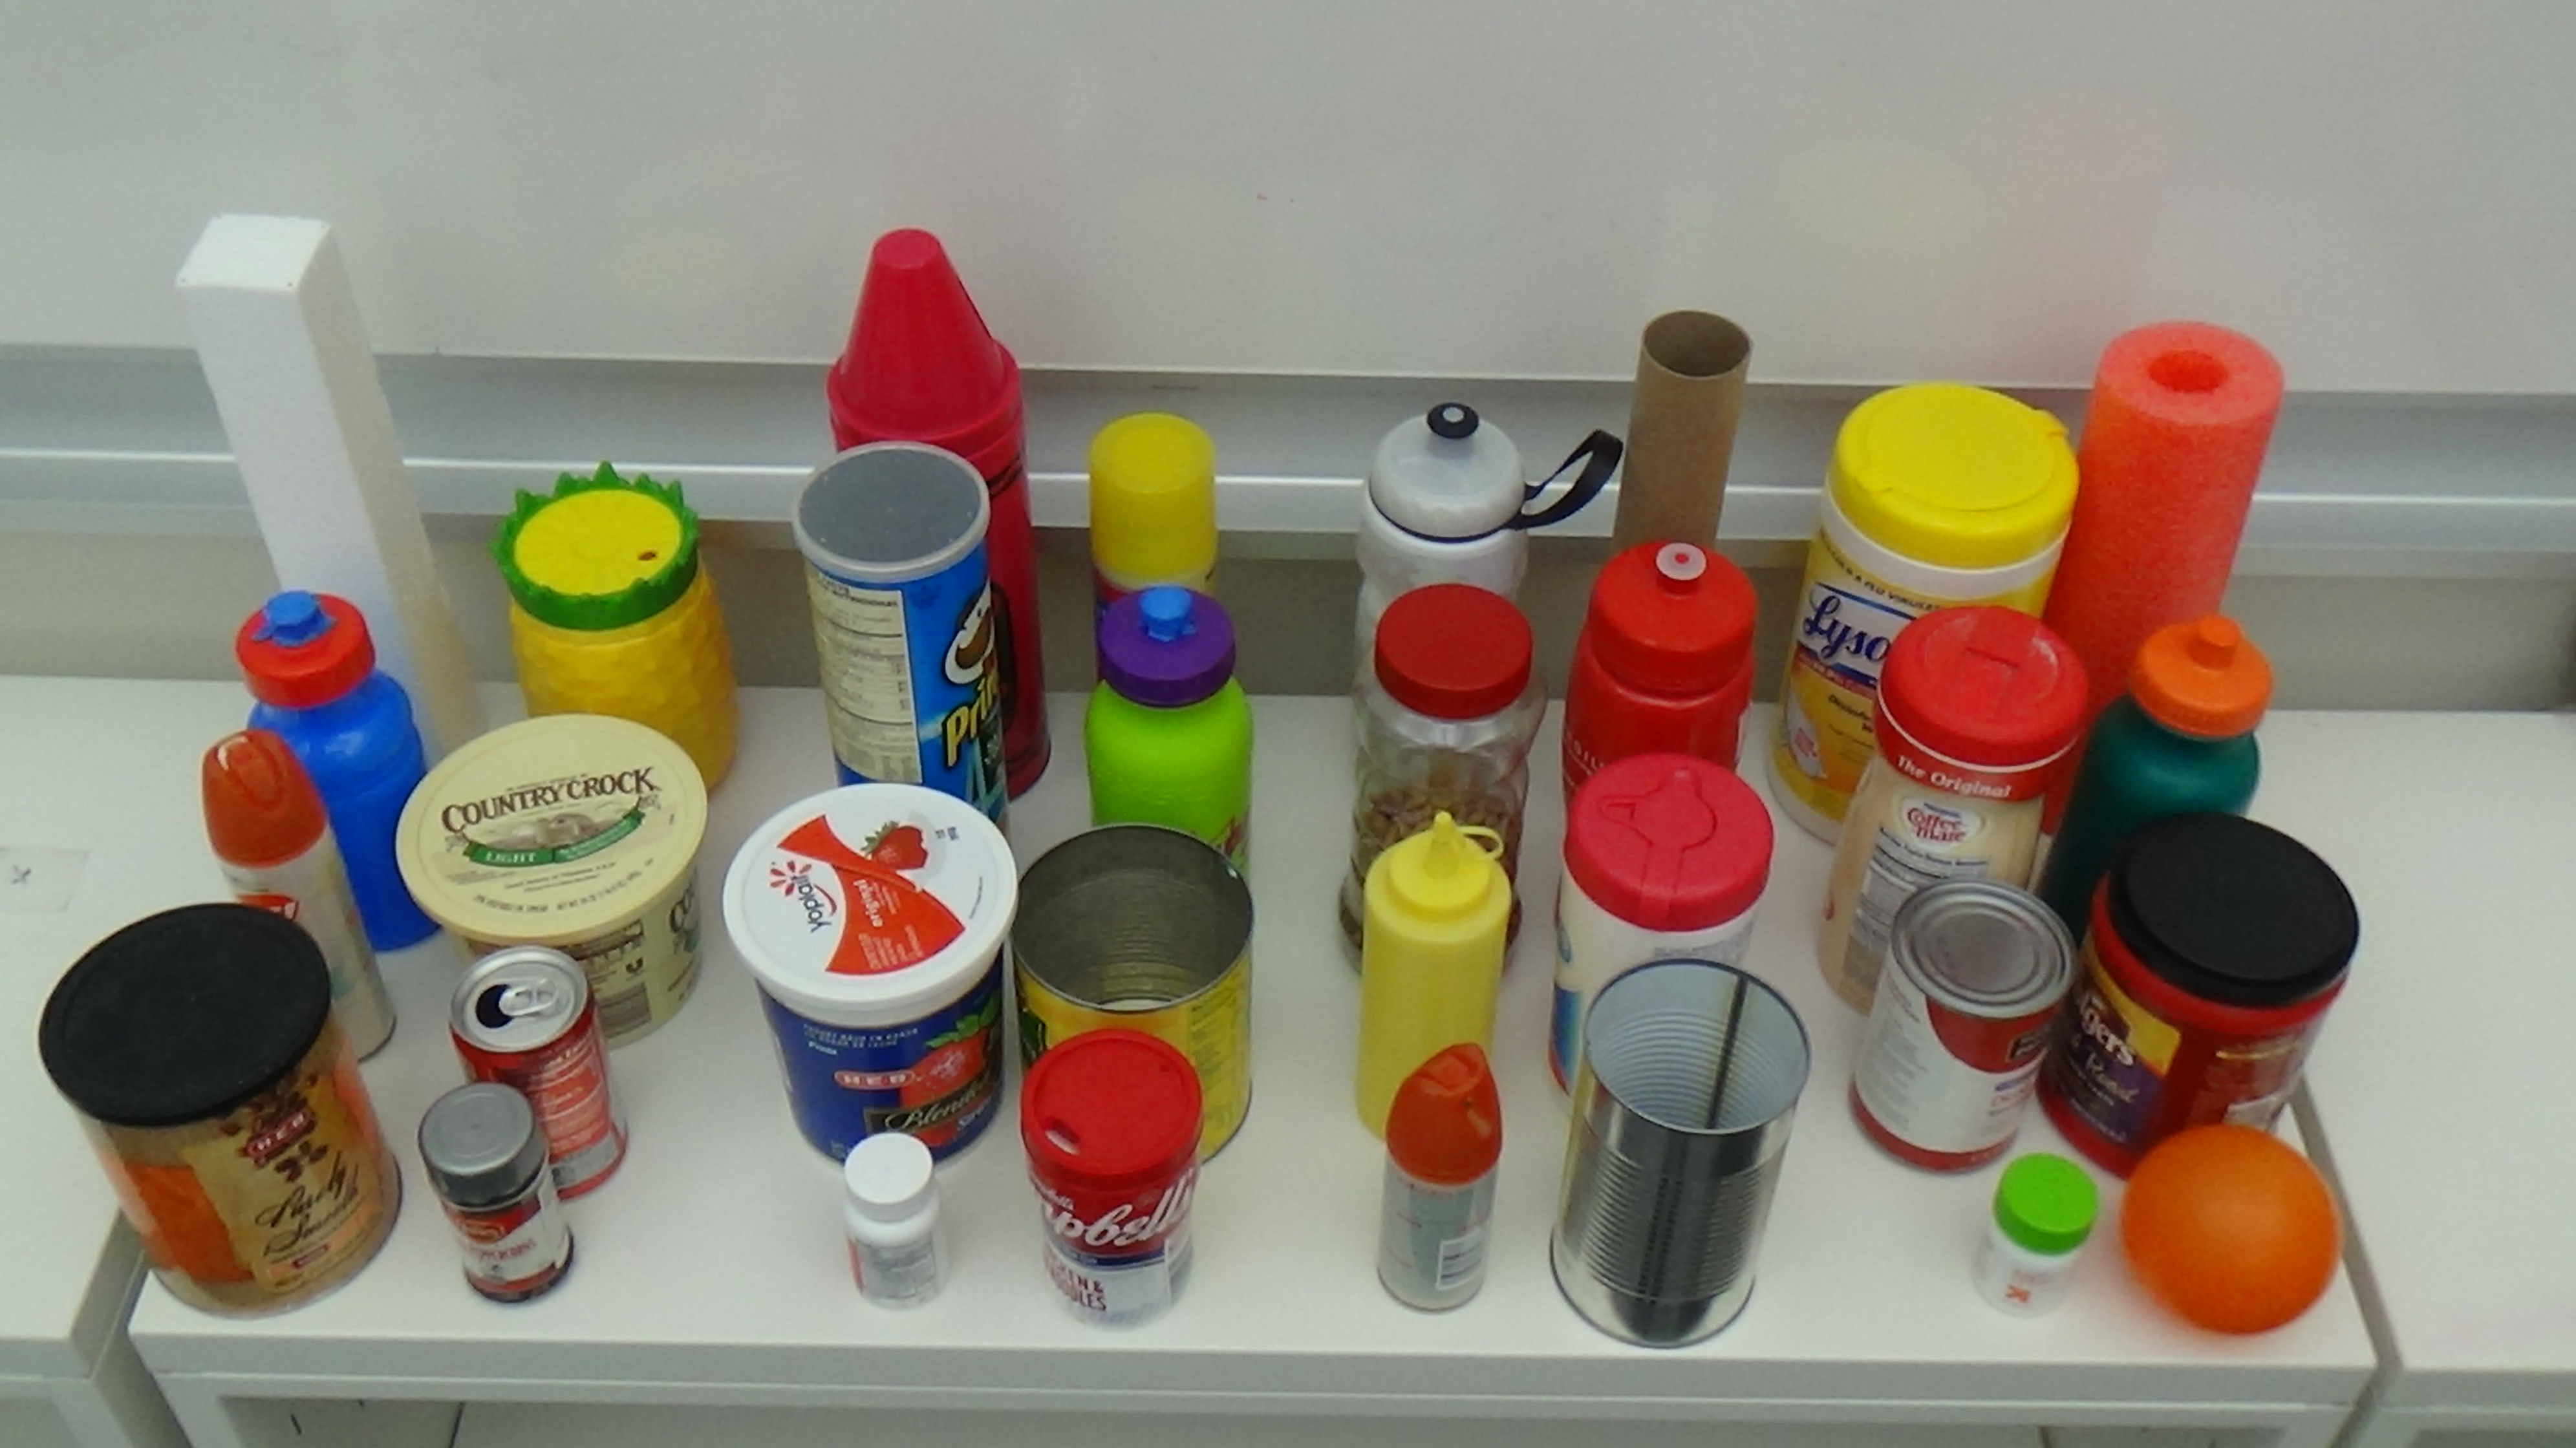
\includegraphics[width=0.3\textwidth]{figures/objects.jpg}
\caption{Objects used in the \ispy game divided into the four folds discussed in Section~\ref{ssec:methodology}, from fold 0 on the left to fold 3 on the right.}
\label{fig:objects}
\end{figure}

The robot used in this study was a Kinova MICO arm mounted on top of a custom-built mobile base.
The robot's sensors included joint effort sensors in each of the robot arm's motors, a microphone mounted on the mobile base, and the Xtion ASUS Pro RGBD camera.
The set of objects used in this experiment consisted of 32 common household items including cups, bottles, cans, and other containers, shown in Figure~\ref{fig:objects}.
Some of the objects contained liquids or other contents (e.g., coffee beans) while others were empty.

\subsection{Exploratory Behaviors and Sensory Modalities}
\label{ssec:contexts}

\begin{center}
\begin{figure}[t]
\setlength{\unitlength}{1in}
 \centerline{
\begin{picture}(3.5,2.5)
\put(0.0,1.4){\psfig{file=figures/behaviors/grasp1.eps,width=1.1in}}
\put(0.4,1.275){grasp}
\put(1.2,1.4){\psfig{file=figures/behaviors/lift1_arrow.eps,width=1.1in}}
\put(1.7,1.275){lift}
\put(2.4,1.4){\psfig{file=figures/behaviors/lower1_arrow.eps,width=1.1in}}
\put(2.8,1.275){lower}
\put(0.0,0.075){\psfig{file=figures/behaviors/drop1.eps,width=1.1in}}
\put(0.45,-0.05){drop}
\put(1.2,0.075){\psfig{file=figures/behaviors/press1_arrow.eps,width=1.1in}}
\put(1.6,-0.05){press}
\put(2.4,0.075){\psfig{file=figures/behaviors/push2_arrow.eps,width=1.1in}}
\put(2.8,-0.05){push}
\end{picture}
}
\caption{The behaviors the robot used to explored the objects. From
left to right and top to bottom: {\it grasp}, {\it lift}, {\it lower},
{\it drop}, {\it press}, and {\it push}. The arrows indicate the
direction of motion of the end-effector for each behavior. In
addition, the {\it hold} behavior (not shown) was performed after the
{\it lift} behavior by simply holding the object in place for half a
second.}
\label{fig:behaviors}
\end{figure}
\end{center}

Prior to the experiment, the robot explored the objects using the methodology described in~\cite{sinapov:ras14}.
In our case, the robot used 7 distinct actions: {\it grasp}, {\it lift}, {\it hold}, {\it lower}, {\it drop}, {\it push}, and {\it press}, shown in Figure~\ref{fig:behaviors}.
During the execution of each action, the robot recorded the sensory perceptions from the {\it haptic} (i.e., joint efforts), {\it proprioceptive} (i.e., joint angular positions), and {\it auditory} sensory modalities.
The joint efforts and joint positions were recorded for all 6 joints at 15 Hz.
The auditory sensory modality was represented as the Discrete Fourrier Transform computed using 65 frequency bins.
To reduce dimensionality of the raw sensory data, we employed the feature extraction methods described in~\cite{sinapov:ras14}. 

In addition to the 7 interactive behaviors, the robot also performed the {\it look} action prior to grasping the object which produced three different kinds of sensory modalities: 1) a color histogram of the object using 8 bins per channel ({\it color}); 2) Fast point feature histogram ({\it fpfh}) shape feautres~\cite{rusu:icra09} as implemented in the Point Cloud Library~\cite{aldoma:ram12}; 3) deep visual features from the 16-layer VGG network~\cite{simonyan:corr14} ({\it vgg}).
The first two types of features were computed using the segmented point cloud of the object while the deep features were computed using the 2D image of the object. 

\begin{table}
\centering
\begin{tabular}[h]{|l|r|r|r|}
	\hline
	\bf Behavior & \multicolumn{3}{c|}{\bf Modality} \\ \hline \hline
	& \bf color & \bf fpfh & \bf vgg \\ \hline
	\bf look & 64 & 308 & 4096 \\ \hline \hline
	& \bf audio & \bf haptics & \bf finger \\ \hline
	\bf grasp & 100 & 60 & 20 \\ \hline
	\bf drop, hold & & & \\
	\bf lift, lower & 100 & 60 & \\
	\bf press, push & & & \\ \hline
\end{tabular}
\caption{The number of features extracted from each \textit{context}, or combination of robot behavior and perceptual modality.}
\label{tab:feature_space_of_contexts}
\end{table}

Thus, each of the robot's 8 actions produced three different kinds of sensory signals.
Each viable combination of an action and a sensory modality is a unique sensorimotor context.
In our experiment, the set of contexts $\mathcal{C}$, was of size  $8 \times 3 = 24$.
The robot performed its full sequence of exploratory actions on each object 5 different times (for the {\it look} behavior, the object was rotated to a new angle each time). Given a context $c \in \mathcal{C}$ and an object $i \in \mathcal{O}$, let the set $\mathcal{X}_i^c$ contain all five feature vectors observed with object $i$ in context $c$.
Table~\ref{tab:feature_space_of_contexts} gives the size of the feature vectors extracted for each context.